% Options for packages loaded elsewhere
\PassOptionsToPackage{unicode}{hyperref}
\PassOptionsToPackage{hyphens}{url}
\PassOptionsToPackage{dvipsnames,svgnames,x11names}{xcolor}
%
\documentclass[
  letterpaper,
  DIV=11,
  numbers=noendperiod]{scrartcl}

\usepackage{amsmath,amssymb}
\usepackage{iftex}
\ifPDFTeX
  \usepackage[T1]{fontenc}
  \usepackage[utf8]{inputenc}
  \usepackage{textcomp} % provide euro and other symbols
\else % if luatex or xetex
  \usepackage{unicode-math}
  \defaultfontfeatures{Scale=MatchLowercase}
  \defaultfontfeatures[\rmfamily]{Ligatures=TeX,Scale=1}
\fi
\usepackage{lmodern}
\ifPDFTeX\else  
    % xetex/luatex font selection
\fi
% Use upquote if available, for straight quotes in verbatim environments
\IfFileExists{upquote.sty}{\usepackage{upquote}}{}
\IfFileExists{microtype.sty}{% use microtype if available
  \usepackage[]{microtype}
  \UseMicrotypeSet[protrusion]{basicmath} % disable protrusion for tt fonts
}{}
\makeatletter
\@ifundefined{KOMAClassName}{% if non-KOMA class
  \IfFileExists{parskip.sty}{%
    \usepackage{parskip}
  }{% else
    \setlength{\parindent}{0pt}
    \setlength{\parskip}{6pt plus 2pt minus 1pt}}
}{% if KOMA class
  \KOMAoptions{parskip=half}}
\makeatother
\usepackage{fancyvrb}
\usepackage{xcolor}
\usepackage[top=25mm,bottom=20mm,left=25mm,right=25mm,heightrounded]{geometry}
\ifLuaTeX
  \usepackage{luacolor}
  \usepackage[soul]{lua-ul}
\else
  \usepackage{soul}
  
\fi
\setlength{\emergencystretch}{3em} % prevent overfull lines
\setcounter{secnumdepth}{3}
% Make \paragraph and \subparagraph free-standing
\ifx\paragraph\undefined\else
  \let\oldparagraph\paragraph
  \renewcommand{\paragraph}[1]{\oldparagraph{#1}\mbox{}}
\fi
\ifx\subparagraph\undefined\else
  \let\oldsubparagraph\subparagraph
  \renewcommand{\subparagraph}[1]{\oldsubparagraph{#1}\mbox{}}
\fi


\providecommand{\tightlist}{%
  \setlength{\itemsep}{0pt}\setlength{\parskip}{0pt}}\usepackage{longtable,booktabs,array}
\usepackage{calc} % for calculating minipage widths
% Correct order of tables after \paragraph or \subparagraph
\usepackage{etoolbox}
\makeatletter
\patchcmd\longtable{\par}{\if@noskipsec\mbox{}\fi\par}{}{}
\makeatother
% Allow footnotes in longtable head/foot
\IfFileExists{footnotehyper.sty}{\usepackage{footnotehyper}}{\usepackage{footnote}}
\makesavenoteenv{longtable}
\usepackage{graphicx}
\makeatletter
\def\maxwidth{\ifdim\Gin@nat@width>\linewidth\linewidth\else\Gin@nat@width\fi}
\def\maxheight{\ifdim\Gin@nat@height>\textheight\textheight\else\Gin@nat@height\fi}
\makeatother
% Scale images if necessary, so that they will not overflow the page
% margins by default, and it is still possible to overwrite the defaults
% using explicit options in \includegraphics[width, height, ...]{}
\setkeys{Gin}{width=\maxwidth,height=\maxheight,keepaspectratio}
% Set default figure placement to htbp
\makeatletter
\def\fps@figure{htbp}
\makeatother
% definitions for citeproc citations
\NewDocumentCommand\citeproctext{}{}
\NewDocumentCommand\citeproc{mm}{%
  \begingroup\def\citeproctext{#2}\cite{#1}\endgroup}
\makeatletter
 % allow citations to break across lines
 \let\@cite@ofmt\@firstofone
 % avoid brackets around text for \cite:
 \def\@biblabel#1{}
 \def\@cite#1#2{{#1\if@tempswa , #2\fi}}
\makeatother
\newlength{\cslhangindent}
\setlength{\cslhangindent}{1.5em}
\newlength{\csllabelwidth}
\setlength{\csllabelwidth}{3em}
\newenvironment{CSLReferences}[2] % #1 hanging-indent, #2 entry-spacing
 {\begin{list}{}{%
  \setlength{\itemindent}{0pt}
  \setlength{\leftmargin}{0pt}
  \setlength{\parsep}{0pt}
  % turn on hanging indent if param 1 is 1
  \ifodd #1
   \setlength{\leftmargin}{\cslhangindent}
   \setlength{\itemindent}{-1\cslhangindent}
  \fi
  % set entry spacing
  \setlength{\itemsep}{#2\baselineskip}}}
 {\end{list}}
\usepackage{calc}
\newcommand{\CSLBlock}[1]{\hfill\break\parbox[t]{\linewidth}{\strut\ignorespaces#1\strut}}
\newcommand{\CSLLeftMargin}[1]{\parbox[t]{\csllabelwidth}{\strut#1\strut}}
\newcommand{\CSLRightInline}[1]{\parbox[t]{\linewidth - \csllabelwidth}{\strut#1\strut}}
\newcommand{\CSLIndent}[1]{\hspace{\cslhangindent}#1}

% This is an UHH LaTeX template for a Quarto PDF document.

% -----------------------------------------------------
% --- FORMAT STYLE FOR KOMA DOCUMENT CLASS SCRARTCL ---
% -----------------------------------------------------


% %----------------------------------------------- General format

\KOMAoptions{paper=a4, pagesize=pdftex}


\usepackage[T1]{fontenc}
\usepackage[utf8]{inputenc}

% Paragraph settings {{{
\setlength{\parindent}{0em}           %  indentation at the first line of a paragraph (here set to 0)
\setlength{\parskip}{0.5em}             % paragraph spacing
\renewcommand{\baselinestretch}{1.0}    % line spacing (here single)
% }}}


% %----------------------------------------------- Fonts

% General {{{
\defaultfontfeatures{Mapping = tex-text}
\setmainfont[BoldFont = font_bold.ttf, ItalicFont = font_italic.ttf, BoldItalicFont = font_bolditalic.ttf]{font_regular.ttf}
\newfontfamily\headingfont[ItalicFont = font_bolditalic.ttf]{font_bold.ttf}
% }}}

% Title and header {{{
\setkomafont{title}{\rmfamily\huge\bfseries}
\setkomafont{subtitle}{\rmfamily\Large}
\setkomafont{author}{\rmfamily\large\bfseries}
\setkomafont{date}{\rmfamily\small\bfseries}
\setkomafont{sectioning}{\rmfamily\large\bfseries}
% }}}

% setting caption text
\usepackage[font=small,labelfont=bf]{caption}



% %----------------------------------------------- Colors

\usepackage{xcolor}				% extends LATEX's color facilities
\usepackage{colortbl}			% to add colour to LaTeX tables
\usepackage{hyperref}			% to handle cross-referencing commands in LaTeX
\PassOptionsToPackage{dvipsnames,svgnames*,x11names*}{xcolor} % for colorlinks

% Define colors for headers and links: {{{
\definecolor{bluegray}{HTML}{3B515B} 
\definecolor{blue}{HTML}{0271BB} 
% }}}

% Font colors {{{
\addtokomafont{title}{\color{bluegray}}           % text color for title
\addtokomafont{subtitle}{\color{bluegray}}        % text color for subtitle
\addtokomafont{author}{\color{bluegray}}          % text color for author
\addtokomafont{date}{\color{bluegray}}            % text color for date
\addtokomafont{disposition}{\color{bluegray}}     % text color for toc section header
\addtokomafont{section}{\color{blue}}             % text color for section header
\addtokomafont{subsection}{\color{bluegray}}      % text color for subsection header
\addtokomafont{subsubsection}{\color{bluegray}}   % text color for subsubsection header
% }}}

% Hypersetup for links {{{ --> currently not working!
\hypersetup{
colorlinks=true,
linkcolor=linkcol,
filecolor=linkcol,
urlcolor=linkcol,
citecolor=linkcol,
bookmarks=true,
linktocpage=true,
pdfpagemode=UseOutlines
}
% }}}


% %----------------------------------------------- Title page

% Aligning title to the left {{{
\usepackage{xpatch}
\makeatletter
\xpatchcmd{\@maketitle}{\begin{center}}{\begin{flushleft}}{}{}
\xpatchcmd{\@maketitle}{\end{center}}{\end{flushleft}}{}{}
\xpatchcmd{\@maketitle}{\begin{tabular}[t]{c}}{\begin{tabular}[t]{@{}l@{}}}{}{}
\makeatother
% }}}

% Adjust abstract section (full width and left aligned) {{{
\renewenvironment{abstract}
 {\rmfamily\small
  \begin{flushleft}
  \rmfamily\bfseries\color{bluegray} \abstractname\vspace{-0.5em}\vspace{0pt}
  \end{flushleft}
  \list{}{
    \setlength{\leftmargin}{.0cm}
    \setlength{\rightmargin}{\leftmargin}
  }
  \item\relax}
 {\endlist}
% }}}
 
% %----------------------------------------------- Header and footer

% Delete default settings and define your own {{{
\usepackage[headsepline, automark]{scrlayer-scrpage}
\clearpairofpagestyles
\ohead[]{\headmark} 
\ofoot[\pagemark]{\pagemark}
\ifoot[]{
\includegraphics[height=10mm]{logo.png}}
% }}}


% %----------------------------------------------- Lists

\usepackage{enumitem}

% Itemized lists {{{
\renewcommand{\labelitemi}{\tiny\textcolor{blue}{$\blacksquare$}}
\renewcommand{\labelitemii}{\textcolor{bluegray}{$\bullet$}}
\renewcommand{\labelitemiii}{\textcolor{blue}{$\bullet$}}
\renewcommand{\labelitemiv}{\textcolor{bluegray}{$\bullet$}}
% }}}

% Enumerated lists {{{ --> does not work currently
% \renewcommand{\theenumi}{\color{blue}}
% \renewcommand{\theenumii}{\color{bluegray}}
% \renewcommand{\theenumiii}{\textcolor{blue}}
% \renewcommand{\theenumiv}{\textcolor{bluegray}}
% }}}


% %----------------------------------------------- Graphics

\usepackage{graphicx}
\graphicspath{ {images/} } % images have to be in the /image subfolder
\KOMAoption{captions}{tableheading}
\makeatletter
\@ifpackageloaded{tcolorbox}{}{\usepackage[skins,breakable]{tcolorbox}}
\@ifpackageloaded{fontawesome5}{}{\usepackage{fontawesome5}}
\definecolor{quarto-callout-color}{HTML}{909090}
\definecolor{quarto-callout-note-color}{HTML}{0758E5}
\definecolor{quarto-callout-important-color}{HTML}{CC1914}
\definecolor{quarto-callout-warning-color}{HTML}{EB9113}
\definecolor{quarto-callout-tip-color}{HTML}{00A047}
\definecolor{quarto-callout-caution-color}{HTML}{FC5300}
\definecolor{quarto-callout-color-frame}{HTML}{acacac}
\definecolor{quarto-callout-note-color-frame}{HTML}{4582ec}
\definecolor{quarto-callout-important-color-frame}{HTML}{d9534f}
\definecolor{quarto-callout-warning-color-frame}{HTML}{f0ad4e}
\definecolor{quarto-callout-tip-color-frame}{HTML}{02b875}
\definecolor{quarto-callout-caution-color-frame}{HTML}{fd7e14}
\makeatother
\makeatletter
\@ifpackageloaded{caption}{}{\usepackage{caption}}
\AtBeginDocument{%
\ifdefined\contentsname
  \renewcommand*\contentsname{Table of contents}
\else
  \newcommand\contentsname{Table of contents}
\fi
\ifdefined\listfigurename
  \renewcommand*\listfigurename{List of Figures}
\else
  \newcommand\listfigurename{List of Figures}
\fi
\ifdefined\listtablename
  \renewcommand*\listtablename{List of Tables}
\else
  \newcommand\listtablename{List of Tables}
\fi
\ifdefined\figurename
  \renewcommand*\figurename{Figure}
\else
  \newcommand\figurename{Figure}
\fi
\ifdefined\tablename
  \renewcommand*\tablename{Table}
\else
  \newcommand\tablename{Table}
\fi
}
\@ifpackageloaded{float}{}{\usepackage{float}}
\floatstyle{ruled}
\@ifundefined{c@chapter}{\newfloat{codelisting}{h}{lop}}{\newfloat{codelisting}{h}{lop}[chapter]}
\floatname{codelisting}{Listing}
\newcommand*\listoflistings{\listof{codelisting}{List of Listings}}
\makeatother
\makeatletter
\makeatother
\makeatletter
\@ifpackageloaded{caption}{}{\usepackage{caption}}
\@ifpackageloaded{subcaption}{}{\usepackage{subcaption}}
\makeatother
\ifLuaTeX
  \usepackage{selnolig}  % disable illegal ligatures
\fi
\usepackage{bookmark}

\IfFileExists{xurl.sty}{\usepackage{xurl}}{} % add URL line breaks if available
\urlstyle{same} % disable monospaced font for URLs
\VerbatimFootnotes % allow verbatim text in footnotes
\hypersetup{
  pdftitle={Document title},
  pdfauthor={Author name(s)},
  colorlinks=true,
  linkcolor={blue},
  filecolor={Maroon},
  citecolor={Blue},
  urlcolor={Blue},
  pdfcreator={LaTeX via pandoc}}

\title{Document title}
\usepackage{etoolbox}
\makeatletter
\providecommand{\subtitle}[1]{% add subtitle to \maketitle
  \apptocmd{\@title}{\par {\large #1 \par}}{}{}
}
\makeatother
\subtitle{Subtitle of document}
\author{Author name(s)}
\date{2024-03-24}

\begin{document}
\maketitle

\section{Introduction}\label{introduction}

\subsection{YAML header}\label{yaml-header}

Configure the YAML header including the following elements:

\begin{itemize}
\tightlist
\item
  \texttt{title}: Title
\item
  \texttt{subtitle}: Subtitle; remove option completely if you don't
  need a subtitle.
\item
  \texttt{author}: Character of single or multiple author(s)
\item
  \texttt{date}: A date
\item
  \texttt{abstract}: The abstract will be shown right after the title in
  smaller font size.
\item
  \texttt{language}: If language is NOT English refer to th file
  \texttt{custom\_lang.yml} for automatic text in German. If the
  document language is another one, adjust this file.
\item
  \texttt{bibliography}: A path to the bibliography file to use for
  references (BibTeX \texttt{.bib} file). The current file includes 3
  dummy references; either insert your references into this file or
  replace the file with your own.
\item
  \texttt{csl}: The style is provided in the `sage-harvard.csl' file,
  which adopts the
  \href{https://uk.sagepub.com/sites/default/files/sage_harvard_reference_style_0.pdf}{SAGE
  Harvard} reference style. Just leave the file as it is.
\item
  \texttt{format\ -\ pdf}: In this template many of the Quarto options
  for PDF output are listed in the YAML header. If you want to know more
  about these settings I recommend the
  \href{https://quarto.org/docs/reference/formats/pdf.html}{PDF format
  reference} for a complete list of available options. For instance, you
  can adjust the figure and table references with \texttt{fig-title},
  \texttt{tbl-title}, \texttt{fig-prefix}, and \texttt{tbl-prefix}.
\item
  \texttt{execute}: Global options for customizing output from executed
  code are specified within this execute key.
\item
  \texttt{fig-align}: Global settings for figure positioning. For other
  settings see the
  \href{https://quarto.org/docs/reference/formats/pdf.html}{PDF format
  reference}.
\end{itemize}

The default font for this template is `Helvetica' but can be replaced
with the University's own font style `TheSansUHH'. If you are associated
with the UHH you are allowed to use this font. You can choose the font
in the template when running the function, e.g.,
\texttt{UHHformats::create\_quarto\_doc(dirname\ =\ "pdf\_simple\_doc",\ template\ =\ "pdf\_simple",\ font\ =\ "TheSansUHH")}.

\subsection{Code blocks}\label{code-blocks}

Code blocks in Quarto documents are treated in similar way as in
Markdown documents. One important difference is that code chunk options
(in Quarto also called `cell level options') are typically included in
special comments using \texttt{\#\textbar{}} at the top of code chunks
rather than within the line that begins the chunk:

Please note that individual words are separated with a hyphen, not a
dot, followed by a colon, not an equal sign as in R Markdown documents.
Quarto uses this approach to both better accommodate longer options like
\texttt{fig-cap}, \texttt{fig-subcap}, and \texttt{fig-alt} as well as
to make it straightforward to edit chunk options within more structured
editors that don't have an easy way to edit chunk metadata (e.g.~most
traditional notebook UIs).

However, if you prefer it is still possible to include chunk options on
the first line (e.g.~```\{r, echo = FALSE\}) as in R Markdown documents.

\subsection{Callout blocks}\label{callout-blocks}

Quarto provides five different types of callouts that are an excellent
way to draw extra attention to certain concepts.

\begin{tcolorbox}[enhanced jigsaw, toprule=.15mm, colbacktitle=quarto-callout-note-color!10!white, colback=white, rightrule=.15mm, left=2mm, title=\textcolor{quarto-callout-note-color}{\faInfo}\hspace{0.5em}{Note}, colframe=quarto-callout-note-color-frame, breakable, bottomtitle=1mm, opacitybacktitle=0.6, opacityback=0, bottomrule=.15mm, arc=.35mm, coltitle=black, leftrule=.75mm, toptitle=1mm, titlerule=0mm]

The color and icon will be different depending upon the type that you
select. You can choose between: \texttt{note}, \texttt{warning},
\texttt{important}, \texttt{tip}, and \texttt{caution}.

\end{tcolorbox}

\begin{tcolorbox}[enhanced jigsaw, toprule=.15mm, colbacktitle=quarto-callout-tip-color!10!white, colback=white, rightrule=.15mm, left=2mm, title=\textcolor{quarto-callout-tip-color}{\faLightbulb}\hspace{0.5em}{Tip With Caption}, colframe=quarto-callout-tip-color-frame, breakable, bottomtitle=1mm, opacitybacktitle=0.6, opacityback=0, bottomrule=.15mm, arc=.35mm, coltitle=black, leftrule=.75mm, toptitle=1mm, titlerule=0mm]

This is an example of a callout with a caption.

\end{tcolorbox}

\section{Methods}\label{methods}

\subsection{Cross-references}\label{cross-references}

External images and R figures can be referenced with
\texttt{@fig-label}, where `label' is the name of the code chunk. These
label names should not contain underscores to separate words, use
hyphens here instead. Note that figures need to have a caption to be
numbered and for cross-referencing, The caption is also set in the chunk
option with \texttt{\#\textbar{}\ fig-cap:\ "Your\ caption"}.

Tables require similarly a label and table caption for
cross-referencing. But here, the cross-reference contains the prefix
`tbl': \texttt{@tbl-label}.

Cross-references to individual sections can simply be made with the
prefix `sec' and by adding a `\{\#sec-identifier\}' to any heading.

This is for example a cross-reference to Table~\ref{tbl-kable} in
Section~\ref{sec-tables} and a cross-reference to Fig.~\ref{fig-base} in
Section~\ref{sec-figures}.

To create a reference-able code block, add a \#lst-identifier along with
a lst-cap attribute inside the curly braces (see code chunk example
Listing~\ref{lst-codeblock}). Note that the indication of the
programming language requires for this static code block a dot set
before the `r'.

\begin{codelisting}

\caption{\label{lst-codeblock}Example for a referenceable code block}

\centering{

\begin{verbatim}
4+4
\end{verbatim}

}

\end{codelisting}%

\subsection{Mathematical equations}\label{mathematical-equations}

Use mathematics as usual with the dollar sign \texttt{\$} at the
beginning and end of the equation; either in \textbf{inline mode} with
one dollar sign such as \(E = mc^2\) or in \textbf{display mode} with
two dollar signs: \[E = mc^2\]

Important to note: do not leave a space between the `\$' and your
mathematical notation.

Alternatively, you can use LaTeX for more control and when equations are
more complicated. LaTeX equations are also automatically numbered if you
define a label within the equation environment, which is useful if you
have many equations and want to cross-reference them. The equation label
needs to be written with `\#eq:label' before the end of the equation
(see Equation~\ref{eq-mean}):

\begin{equation}\phantomsection\label{eq-mean}{
  \bar{X} = \frac{\sum_{i=1}^n X_i}{n}
}\end{equation}

Formulas and corresponding explanations should be integrated into the
sentence and, thus, end with a comma or period. Here comes an example:

If the random variable \(Y\) follows a standard normal distribution,
i.e.~\(Y \sim N(0,1)\), it's density function can be described with

\begin{equation}\phantomsection\label{eq-density-norm}{
f_{Y}(y)=\varphi(y) \stackrel{\mathrm{def}}{=} \frac{1}{\sqrt{2 \pi}} \exp \left\{ -\frac{y^2}{2} \right\}, \quad y \in \mathbb{R}.
}\end{equation}

\(\pi\) represents the circle number or Ludolph's number. The function

\begin{equation}\phantomsection\label{eq-dist-func}{
  F_{Y}(y)=\Phi(y) \stackrel{\mathrm{def}}{=} \int_{-\infty}^y \varphi(x) \,\mathrm{d}x, \quad y \in \mathbb{R}
}\end{equation}

represents then the distribution function of
Equation~\ref{eq-density-norm}.

The numbering of equations, as in Equation~\ref{eq-density-norm}, should
only be done if they are referred to in the rest of the text. Especially
if there are many equations in the thesis, the use of LaTeX seems to
make more sense.

\subsection{Images}\label{images}

Quarto includes several features aimed at making it easier to work with
figures and subfigures, as well as for laying out panels that contain
multiple figures, tables, or other content.

\begin{figure}[H]

{\centering 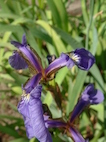
\includegraphics{images/wikipedia_iris_setosa.jpg}

}

\caption{Single image of Iris setosa with URL link but no
cross-reference.}

\end{figure}%

For instance, if you have several figures that appear as a group, you
can create a figure div to enclose them (see Fig.~\ref{fig-versicolor}
and Fig.~\ref{fig-virginica}).

\begin{figure}

\begin{minipage}{0.50\linewidth}

\begin{figure}[H]

\centering{

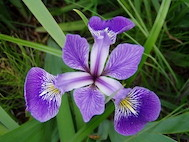
\includegraphics{images/wikipedia_iris_versicolor.jpg}

}

\caption{\label{fig-versicolor}Iris versicolor}

\end{figure}%

\end{minipage}%
%
\begin{minipage}{0.50\linewidth}

\begin{figure}[H]

\centering{

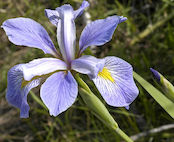
\includegraphics{images/wikipedia_iris_virginica.jpg}

}

\caption{\label{fig-virginica}Iris virginica}

\end{figure}%

\end{minipage}%

\end{figure}%

The layout attribute enables the creation of much more complex layouts.
Fig.~\ref{fig-custom-layout} provides an example with a common figure
caption and one identifier for all three.

\begin{figure}

\begin{minipage}{0.20\linewidth}

\begin{figure}[H]

{\centering 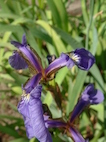
\includegraphics{images/wikipedia_iris_setosa.jpg}

}

\subcaption{Iris setosa}

\end{figure}%

\end{minipage}%
%
\begin{minipage}{0.02\linewidth}
~\end{minipage}%
%
\begin{minipage}{0.46\linewidth}

\begin{figure}[H]

{\centering 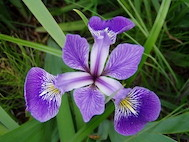
\includegraphics{images/wikipedia_iris_versicolor.jpg}

}

\subcaption{Iris versicolor}

\end{figure}%

\end{minipage}%
%
\begin{minipage}{0.02\linewidth}
~\end{minipage}%
%
\begin{minipage}{0.30\linewidth}

\begin{figure}[H]

{\centering 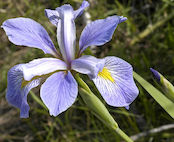
\includegraphics{images/wikipedia_iris_virginica.jpg}

}

\subcaption{Iris virginica}

\end{figure}%

\end{minipage}%

\caption{\label{fig-custom-layout}Custom layout of images}

\end{figure}%

\newpage

\section{Results}\label{results}

\subsection{R output}\label{r-output}

R output is typically shown in the monospace font (here an example with
the \texttt{mtcars} dataset in the subfolder \texttt{data/}):

\begin{verbatim}
      mpg             cyl             disp             hp       
 Min.   :10.40   Min.   :4.000   Min.   : 71.1   Min.   : 52.0  
 1st Qu.:15.43   1st Qu.:4.000   1st Qu.:120.8   1st Qu.: 96.5  
 Median :19.20   Median :6.000   Median :196.3   Median :123.0  
 Mean   :20.09   Mean   :6.188   Mean   :230.7   Mean   :146.7  
 3rd Qu.:22.80   3rd Qu.:8.000   3rd Qu.:326.0   3rd Qu.:180.0  
 Max.   :33.90   Max.   :8.000   Max.   :472.0   Max.   :335.0  
\end{verbatim}

\subsection{Tables}\label{sec-tables}

Here is a simple table based on Markdown Syntax
(Table~\ref{tbl-markdown}).

\begin{longtable}[]{@{}lcr@{}}
\caption{My Caption}\label{tbl-markdown}\tabularnewline
\toprule\noalign{}
A & New & Table \\
\midrule\noalign{}
\endfirsthead
\toprule\noalign{}
A & New & Table \\
\midrule\noalign{}
\endhead
\bottomrule\noalign{}
\endlastfoot
left-aligned & center-aligned & right-aligned \\
\$123 & \$456 & \$789 \\
\emph{italics} & \st{strikethrough} & \textbf{boldface} \\
\end{longtable}

\subsubsection{\texorpdfstring{Using the \emph{knitr}
package}{Using the knitr package}}\label{using-the-knitr-package}

Table~\ref{tbl-kable} is an example of using \texttt{knitr::kable()} to
generate the table.

\begin{longtable}[]{@{}lrrrrrr@{}}

\caption{\label{tbl-kable}This is a table produced with knitr::kable().}

\tabularnewline

\toprule\noalign{}
& mpg & cyl & disp & hp & drat & wt \\
\midrule\noalign{}
\endhead
\bottomrule\noalign{}
\endlastfoot
Mazda RX4 & 21.0 & 6 & 160 & 110 & 3.90 & 2.620 \\
Mazda RX4 Wag & 21.0 & 6 & 160 & 110 & 3.90 & 2.875 \\
Datsun 710 & 22.8 & 4 & 108 & 93 & 3.85 & 2.320 \\
Hornet 4 Drive & 21.4 & 6 & 258 & 110 & 3.08 & 3.215 \\
Hornet Sportabout & 18.7 & 8 & 360 & 175 & 3.15 & 3.440 \\

\end{longtable}

\subsubsection{\texorpdfstring{The \emph{xtable}
package}{The xtable package}}\label{the-xtable-package}

Another useful package for tables for PDF output is
\href{https://cran.r-project.org/web/packages/xtable/vignettes/xtableGallery.pdf}{xtable}.
The following code will produce an example table if the \emph{xtable}
package is installed. Note that you need to add the chunk option
\texttt{results\ =\ "asis"} inside \texttt{\{r\}} otherwise the PDF will
contain the \LaTeX code of the table!

\begin{table}

\caption{\label{tbl-xtable}A table made with xtable.}

\centering{

[ht]
\centering
\begin{tabular}{rrrrrrr}
  \toprule
 & mpg & cyl & disp & hp & drat & wt \\ 
  \midrule
Mazda RX4 & 21.00 &   6 & 160.00 & 110 & 3.90 & 2.62 \\ 
  Mazda RX4 Wag & 21.00 &   6 & 160.00 & 110 & 3.90 & 2.88 \\ 
  Datsun 710 & 22.80 &   4 & 108.00 &  93 & 3.85 & 2.32 \\ 
  Hornet 4 Drive & 21.40 &   6 & 258.00 & 110 & 3.08 & 3.21 \\ 
  Hornet Sportabout & 18.70 &   8 & 360.00 & 175 & 3.15 & 3.44 \\ 
   \bottomrule
\end{tabular}

}

\end{table}%

\subsection{Figures}\label{sec-figures}

A base graphics scatterplot (Fig.~\ref{fig-base}).

\begin{figure}

\centering{

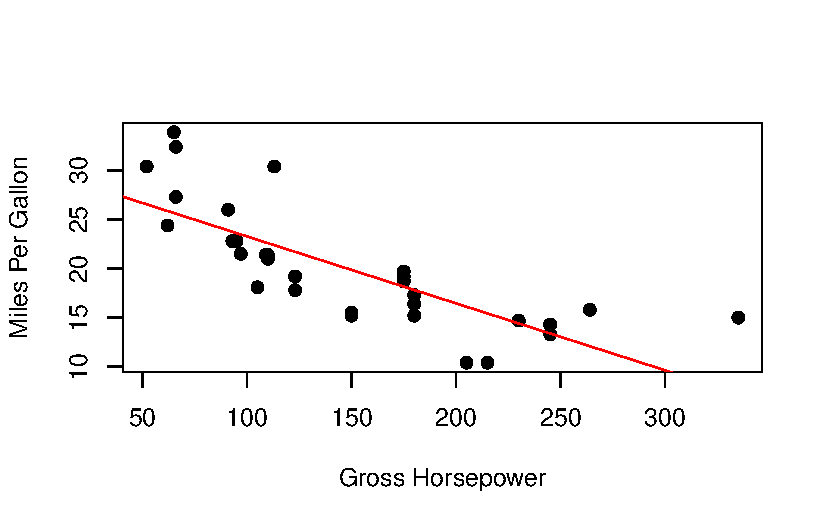
\includegraphics{simple_pdf_UHH_template_files/figure-pdf/fig-base-1.pdf}

}

\caption{\label{fig-base}Relationship between horsepower and fuel
economy.}

\end{figure}%

Here for comparison a boxplot with a different image height
(Fig.~\ref{fig-boxplot}).

\begin{figure}

\centering{

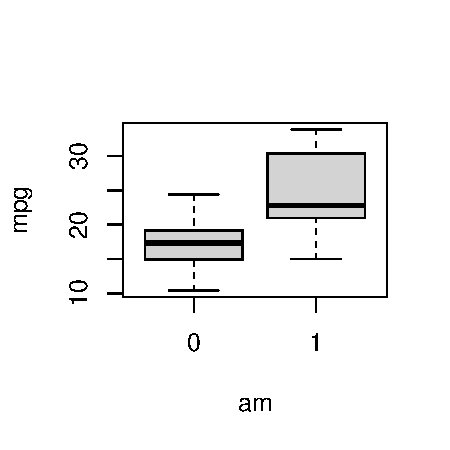
\includegraphics{simple_pdf_UHH_template_files/figure-pdf/fig-boxplot-1.pdf}

}

\caption{\label{fig-boxplot}Fuel differences between transmission types
(0 = automatic, 1 = manual).}

\end{figure}%

\subsection{Diagrams}\label{diagrams}

Quarto has native support for embedding \emph{Mermaid} and
\emph{Graphviz} diagrams. This enables you to create flowcharts,
sequence diagrams, state diagrams, gnatt charts, and more using a plain
text syntax inspired by markdown.

\subsubsection{Mermaid}\label{mermaid}

Mermaid is a Javascript based diagramming and charting tool that uses
Markdown-inspired text definitions and a renderer to create and modify
complex diagrams (see Fig.~\ref{fig-mermaid-diagram}).

\begin{figure}

\centering{

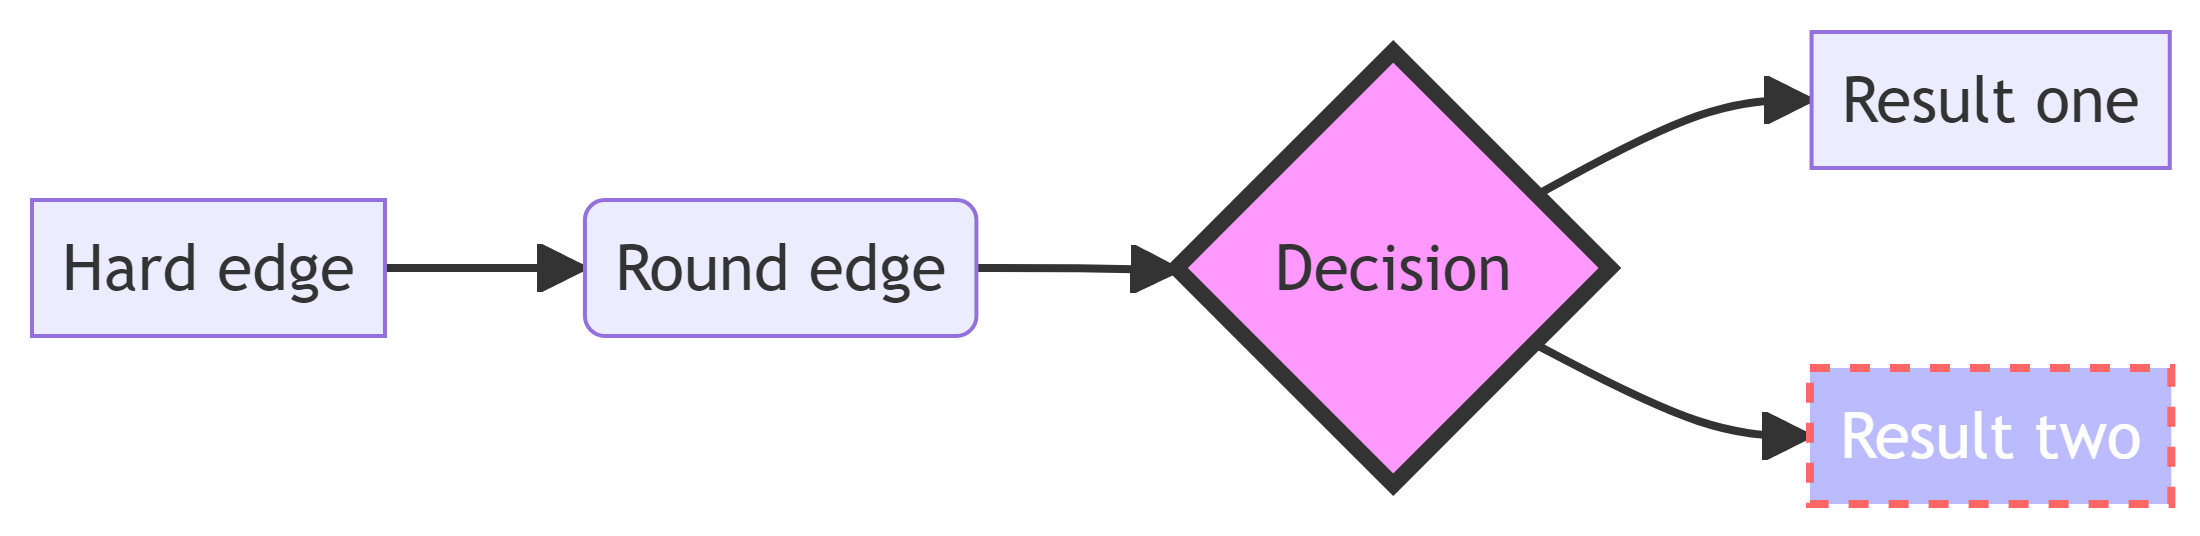
\includegraphics[width=6in,height=1.46in]{simple_pdf_UHH_template_files/figure-latex/mermaid-figure-1.png}

}

\caption{\label{fig-mermaid-diagram}Simple flowchart based on the
JS-tool Mermaid.}

\end{figure}%

\begin{tcolorbox}[enhanced jigsaw, toprule=.15mm, colbacktitle=quarto-callout-note-color!10!white, colback=white, rightrule=.15mm, left=2mm, title=\textcolor{quarto-callout-note-color}{\faInfo}\hspace{0.5em}{Note}, colframe=quarto-callout-note-color-frame, breakable, bottomtitle=1mm, opacitybacktitle=0.6, opacityback=0, bottomrule=.15mm, arc=.35mm, coltitle=black, leftrule=.75mm, toptitle=1mm, titlerule=0mm]

Cell level options are here indicated with \texttt{\%\%\textbar{}}
instead of \texttt{\#\textbar{}}!

\end{tcolorbox}

Useful links:

\begin{itemize}
\tightlist
\item
  \url{https://mermaid-js.github.io/mermaid/\#/}
\item
  \url{https://mermaid.live}
\end{itemize}

\subsubsection{Graphviz}\label{graphviz}

The \href{https://graphviz.org/}{Graphviz} layout programs take
descriptions of graphs in a simple text language and make diagrams in
useful formats. Graphviz has many useful features for concrete diagrams,
such as options for colors, fonts, tabular node layouts, line styles,
hyperlinks, and custom shapes (see Fig.~\ref{fig-dot-diagram}).

\begin{figure}

\centering{

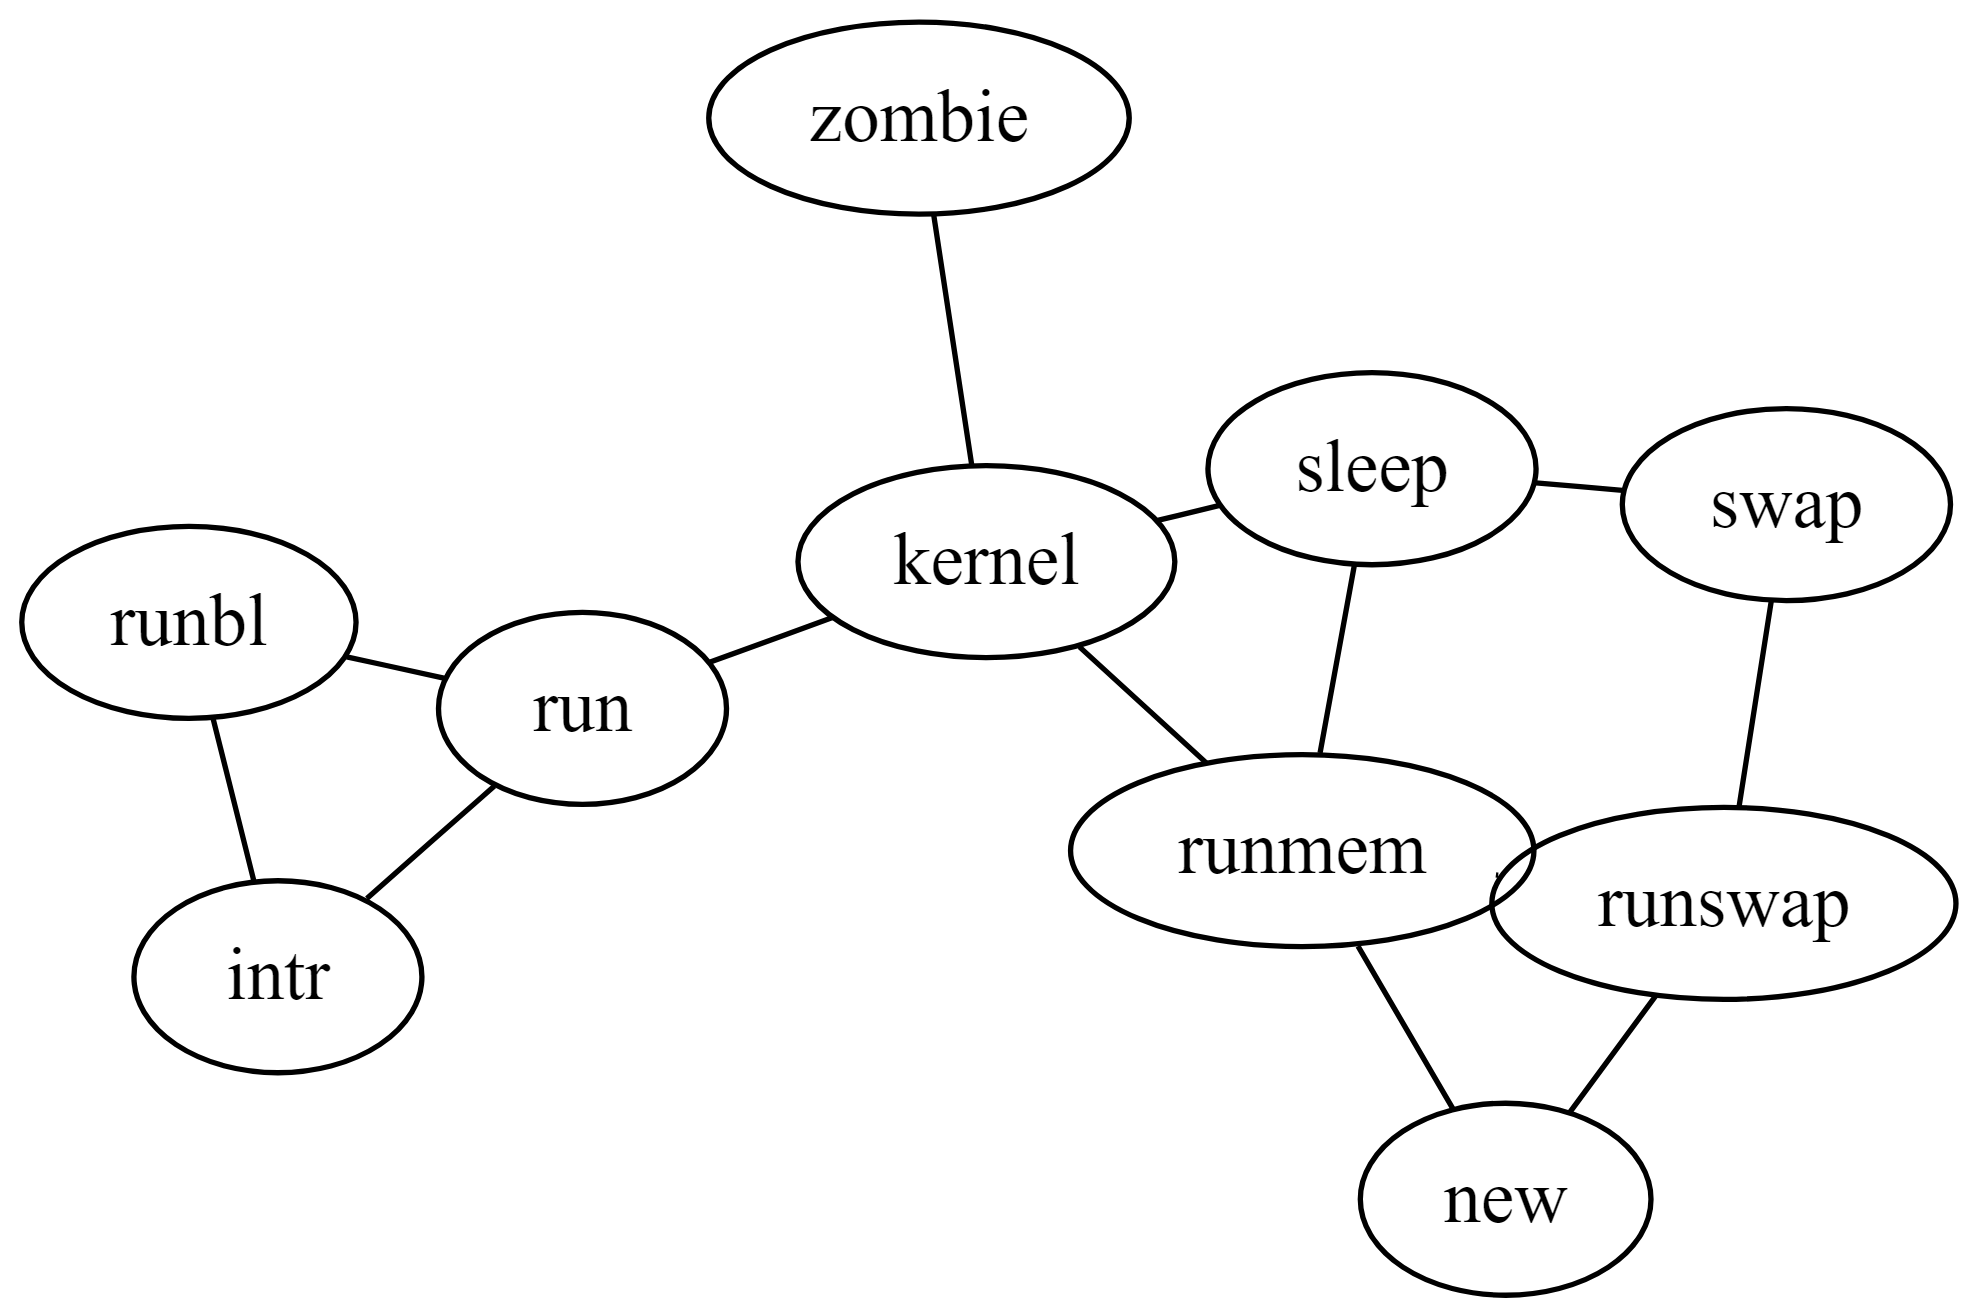
\includegraphics[width=5.5in,height=3.5in]{simple_pdf_UHH_template_files/figure-latex/dot-figure-1.png}

}

\caption{\label{fig-dot-diagram}An example for a diagram made with
Graphviz.}

\end{figure}%

\begin{tcolorbox}[enhanced jigsaw, toprule=.15mm, colbacktitle=quarto-callout-note-color!10!white, colback=white, rightrule=.15mm, left=2mm, title=\textcolor{quarto-callout-note-color}{\faInfo}\hspace{0.5em}{Note}, colframe=quarto-callout-note-color-frame, breakable, bottomtitle=1mm, opacitybacktitle=0.6, opacityback=0, bottomrule=.15mm, arc=.35mm, coltitle=black, leftrule=.75mm, toptitle=1mm, titlerule=0mm]

Cell level options are here indicated with \texttt{//\textbar{}}!

\end{tcolorbox}

\section{Adding citations and
bibliography}\label{adding-citations-and-bibliography}

Link a \texttt{.bib} document via the YAML header, and the bibliography
will be printed at the end. The default bibliography style is provided
in the \texttt{sage-harvard.csl} file (do not delete), which adopts the
\href{https://uk.sagepub.com/sites/default/files/sage_harvard_reference_style_0.pdf}{SAGE
Harvard} reference style.

References can be cited directly within the document using the Quarto
equivalent of the \LaTeX citation system \texttt{{[}@key{]}}, where key
is the citation key in the first line of the entry in the .csl file.
Example: (Taylor and Green, 1937). To cite multiple entries, separate
the keys by semicolons (e.g., (Kamm, 2000; Knupp, 1999). You can also
write in-text citations, as follows: Taylor and Green (1937) say this
and that.

There is also the package \href{https://github.com/crsh/citr}{citr}
which I highly recommend: \emph{citr} provides functions and an RStudio
add-in to search a BibTeX-file to create and insert formatted Markdown
citations into the current document. If you are using the reference
manager \href{https://www.zotero.org/}{Zotero} the add-in can access
your reference database directly.

\subsection{Software}\label{software}

If you want to include a paragraph on the software used, here is some
example text/code to get the current R and package versions. The code to
create a separate bibliography file named `packages.bib' with all
package references has already been added at the beginning of this
script (code chunk `generate-package-refs').

All analyses were performed using the statistical software R (version
4.3.1) (R Core Team, 2023). This thesis, including tables, was generated
using the R packages `rmarkdown' (version 2.26) (Allaire et al., 2024),
`UHHformats' (version 1.0.0.9000) (Otto, 2022), and `knitr' (version
1.45) (Xie, 2023).

\subsection{Examples for footnotes}\label{examples-for-footnotes}

Here is a footnote reference\footnote{Here is the footnote.}, and
another\footnote{Here's one with multiple blocks.

  Subsequent paragraphs are indented to show that they belong to the
  previous footnote.

\begin{Verbatim}
{ some.code }
\end{Verbatim}

  The whole paragraph can be indented, or just the first line. In this
  way, multi-paragraph footnotes work like multi-paragraph list items.}.

\newpage

\section{References}\label{references}

\phantomsection\label{refs}
\begin{CSLReferences}{1}{1}
\bibitem[\citeproctext]{ref-R-rmarkdown}
Allaire J, Xie Y, Dervieux C, et al. (2024) \emph{Rmarkdown: Dynamic
Documents for r}. Available at:
\url{https://github.com/rstudio/rmarkdown}.

\bibitem[\citeproctext]{ref-Kamm2000}
Kamm J (2000) \emph{Evaluation of the {S}edov-von {N}eumann-{T}aylor
blast wave solution}. Technical {R}eport LA-UR-00-6055. Los {A}lamos
{N}ational {L}aboratory.

\bibitem[\citeproctext]{ref-Knupp1999}
Knupp P (1999) Winslow smoothing on two-dimensional unstructured meshes.
\emph{Eng {C}omput} 15: 263--268.

\bibitem[\citeproctext]{ref-R-UHHformats}
Otto S (2022) \emph{UHHformats: Templates for HTML and PDF/LaTeX Output
Formats Designed for the UHH}. Available at:
\url{https://github.com/uham-bio/UHHformats}.

\bibitem[\citeproctext]{ref-R-base}
R Core Team (2023) \emph{R: A Language and Environment for Statistical
Computing}. Vienna, Austria: R Foundation for Statistical Computing.
Available at: \url{https://www.R-project.org/}.

\bibitem[\citeproctext]{ref-Taylor1937}
Taylor G and Green A (1937) Mechanism of the production of small eddies
from large ones. \emph{P {R}oy {S}oc {L}ond {A} {M}at} 158(895):
499--521.

\bibitem[\citeproctext]{ref-R-knitr}
Xie Y (2023) \emph{Knitr: A General-Purpose Package for Dynamic Report
Generation in r}. Available at: \url{https://yihui.org/knitr/}.

\end{CSLReferences}

\section*{Acknowledgments}\label{acknowledgments}

Lorem ipsum dolor sit amet, consectetur adipiscing elit. Aenean ut elit
odio. Donec fermentum tellus neque, vitae fringilla orci pretium vitae.
Fusce maximus finibus facilisis. Donec ut ullamcorper turpis.



\end{document}
